%%%%%%%%%%%%%%%%%%%%%%%%%%%%%%%%%%%%%%%%%%%%%%%%%%%%%%%%%%%%%%%%%%%%%%%%
\section{Problem 2: EBMs on MNIST (40 points)}
%%%%%%%%%%%%%%%%%%%%%%%%%%%%%%%%%%%%%%%%%%%%%%%%%%%%%%%%%%%%%%%%%%%%%%%%

\begin{question}
You will implement an Energy Based Model and evaluate it for generative performance and anomaly detection capacity, using the notebook \texttt{ebm-mnist.ipynb}.
\begin{enumerate}
  \item[(a)] Part 0/1: Libraries and utility functions. How does the contrastive divergence objective change the energy of the correct/wrong samples? What do you think would need to happen for the push/pull forces on the diagram to balance out?
  \item[(b)] Part 2: Model construction and training. Implement the model construction, MCMC sampling steps, and loss calculation, and run the implemented model.
  \begin{itemize}
    \item Why do you think that the Swish activation function is more convenient than the standard ReLU for this model and task? \emph{Hint: visualize both activation functions and think about how they would affect the backward propagation of the gradient through the network.}
    \item What is the role of the regularization loss? How do you think the resulting data would look if we were not using it?
  \end{itemize}
  \item[(c)] Part 3: Analysis. Sample a few images using the MCMC method. How many MCMC steps are required to sample reasonable images from the trained model? Is this number different for different digits? Then complete the transformation cells to test the out-of-distribution performance of the model.
  \begin{itemize}
    \item For pure random noise inputs: are the scores in line with what would be expected for a good anomaly detection method? Why do you think the score for the `true' images is so close to zero?
    \item For the image transformations: do the scores of the transformed images differ significantly from the original ones? Do you think this model would make a good out-of-distribution detector? Provide a detailed explanation of why this would or would not be the case.
  \end{itemize}
\end{enumerate}
\end{question}

The network outputs a scalar score \(f_\theta(x)\), and the notebook defines the model density as
\begin{equation}
  q_\theta(x) = \frac{\exp\bigl(f_\theta(x)\bigr)}{Z_\theta},
  \qquad
  f_\theta(x) = -E_\theta(x),
  \label{eq:ebm-q}
\end{equation}
so a high score means low energy and high unnormalized probability. The normalizer \(Z_\theta\) integrates \(\exp(f_\theta)\) over all images and is intractable. Images are scaled to \([-1,1]\), which is also the box the sampler is clipped to.

\subsection{Part 0/1: Contrastive divergence}

Maximum likelihood minimizes \(\mathcal{L}(\theta) = -\mathbb{E}_{p(x)}[\log q_\theta(x)]\). Since \(\log q_\theta(x) = f_\theta(x) - \log Z_\theta\) and \(\nabla_\theta \log Z_\theta = \mathbb{E}_{q_\theta(x)}[\nabla_\theta f_\theta(x)]\),
\begin{equation}
  \nabla_\theta \mathcal{L}
  = \mathbb{E}_{q_\theta(x)}\bigl[\nabla_\theta f_\theta(x)\bigr]
  - \mathbb{E}_{p(x)}\bigl[\nabla_\theta f_\theta(x)\bigr].
  \label{eq:cd-grad}
\end{equation}
A descent step therefore raises \(f_\theta\) on data and lowers it on model samples. In energy terms, that is the pair of forces in the diagram.

\subsubsection{Effect on the energy of correct and wrong samples}

The ``correct answer'' is a training image \(x_{\mathrm{train}} \sim p(x)\); the update lowers its energy, pulling it down the energy curve and making it more probable. The ``wrong answer'' is a model sample \(x_{\mathrm{sample}} \sim q_\theta(x)\); the update raises its energy and makes it less probable. Replacing the model expectation with one sample gives the contrastive divergence loss used later,
\begin{equation}
  \ell_{\mathrm{CD}} = f_\theta(x_{\mathrm{sample}}) - f_\theta(x_{\mathrm{train}})
  = E_\theta(x_{\mathrm{train}}) - E_\theta(x_{\mathrm{sample}}),
  \label{eq:cd-loss}
\end{equation}
and minimizing it is the same push and pull: down on data, up on samples.

\subsubsection{When the push and pull balance}

The gradient~\eqref{eq:cd-grad} vanishes when \(\mathbb{E}_{p}[\nabla_\theta f_\theta] = \mathbb{E}_{q_\theta}[\nabla_\theta f_\theta]\), which holds once \(q_\theta = p\). Model samples then land on the same images as the training data, so the upward push on ``wrong'' samples and the downward pull on ``correct'' ones act on the same regions and cancel. Until then, mass sitting off the data keeps being pushed up and real digits keep being pulled down.

\subsection{Part 2: Model construction and training}

\subsubsection{Energy network}

\(f_\theta\) is a small CNN with Swish activations, \(x\,\sigma(x)\). On a \(1\times 28\times 28\) image:
\begin{center}
\begin{tabular}{lll}
\toprule
Layer & Shape & Activation \\
\midrule
Conv \(5\times 5\), stride 2, pad 4 & \(1 \to 16\), \(16\times 16\) & Swish \\
Conv \(3\times 3\), stride 2, pad 1 & \(16 \to 32\), \(8\times 8\) & Swish \\
Conv \(3\times 3\), stride 2, pad 1 & \(32 \to 64\), \(4\times 4\) & Swish \\
Conv \(3\times 3\), stride 2, pad 1 & \(64 \to 64\), \(2\times 2\) & Swish \\
Flatten & \(256\) & none \\
Linear & \(256 \to 64\) & Swish \\
Linear & \(64 \to 1\) & none \\
\bottomrule
\end{tabular}
\end{center}
The output is squeezed to one score \(f_\theta(x) = -E_\theta(x)\) per image. The network has \(76{,}993\) parameters.

\subsubsection{Langevin sampler}

Samples come from short-run Langevin dynamics in the box \([-1,1]\). Each of \(K\) steps, with step size \(\nu\), is
\begin{align}
  x &\leftarrow \mathrm{clip}\bigl(x + \omega,\, -1,\, 1\bigr),
  & \omega &\sim \mathcal{N}(0,\, 0.005^{2}), \nonumber \\
  g &\leftarrow \mathrm{clip}\bigl(\nabla_x E_\theta(x),\, -0.03,\, 0.03\bigr), \nonumber \\
  x &\leftarrow \mathrm{clip}\bigl(x - \nu g,\, -1,\, 1\bigr).
  \label{eq:langevin}
\end{align}
The gradient of \(E_\theta = -f_\theta\) is taken with the weights frozen and clipped so a single step cannot jump across the image; \(x - \nu g\) walks downhill in energy. Training uses \(K = 60\) and \(\nu = 10\). The generation plots use \(K = 256\) from fresh noise.

A replay buffer of up to \(8{,}192\) images supplies the starting points: \(95\%\) of each batch comes from the buffer and \(5\%\) from fresh uniform noise, and the new samples go to the front of the buffer. These warm starts are why \(60\) steps suffice during training, since most chains already start near a mode.

\subsubsection{Loss}

Real images get pixel noise with standard deviation \(0.005\) and are clipped back to \([-1,1]\). The network scores the real and sampled batches together, and with \(f_{\mathrm{real}}\), \(f_{\mathrm{fake}}\) those scores,
\begin{align}
  \ell_{\mathrm{CD}} &= \mathbb{E}[f_{\mathrm{fake}}] - \mathbb{E}[f_{\mathrm{real}}], \\
  \ell_{\mathrm{reg}} &= \mathbb{E}\bigl[f_{\mathrm{real}}^{2} + f_{\mathrm{fake}}^{2}\bigr], \\
  \ell &= \ell_{\mathrm{CD}} + \alpha\,\ell_{\mathrm{reg}},
  \qquad \alpha = 0.1.
  \label{eq:ebm-loss}
\end{align}
\(\ell_{\mathrm{CD}}\) is the batch version of~\eqref{eq:cd-loss}. The optimizer is Adam with learning rate \(10^{-4}\) and betas \((0, 0.999)\); first-moment momentum is off because the loss surface moves as the negative samples change. The learning rate decays by \(0.97\) per epoch, and gradients are clipped to global norm \(0.1\). The model was trained for the full \(60\) epochs with batch size \(128\) on a single NVIDIA H100 on PACE ICE. The checkpoint used below is the best one by validation contrastive divergence, from epoch \(58\) (counting from \(0\), so the \(59\)th of \(60\)) at step \(27{,}612\).

\subsubsection{Swish vs.\ ReLU}

Swish is smooth: for positive inputs it approaches \(y = x\), and for negative inputs it dips slightly below zero and returns toward it. Its derivative,
\[
  \sigma(x)\bigl(1 + x\bigl(1-\sigma(x)\bigr)\bigr),
\]
is continuous and is zero only at the single point \(x \approx -1.28\). ReLU's derivative is exactly zero on all of \(x < 0\) and jumps at the origin.

That matters because sampling follows \(\nabla_x f_\theta(x)\), which has to backpropagate through every activation. Wherever a ReLU unit is off, that part of the energy surface is flat, the input gradient dies, and the Langevin chain stalls. Swish still passes a slope through those regions, so both the sampler and the parameter updates keep a direction. ReLU's kink also makes \(\nabla_x f_\theta\) discontinuous, which makes Langevin steps jumpy; Swish keeps \(f_\theta\) smooth.

\subsubsection{Role of the regularization loss}

Contrastive divergence only sees the gap \(f_{\mathrm{fake}} - f_{\mathrm{real}}\). That gap can grow without bound by sending real scores to \(+\infty\) and fake scores to \(-\infty\), which doesn't change which images are relatively likely but turns the energy surface into a cliff. Langevin steps would then always hit the \(\pm 0.03\) gradient cap and slam into the \(\pm 1\) walls, the samples would become saturated noise or harsh blobs, and training would diverge.

The penalty \(\alpha\,\mathbb{E}[f_{\mathrm{real}}^{2} + f_{\mathrm{fake}}^{2}]\) keeps both scores near zero, so training has to shape the surface rather than just stretch it. It is also why real-image scores sit near zero in Part~3: zero is the scale the regularizer picked, not a statement that the probability is \(1\).

\subsection{Part 3: Analysis}

Everything below uses that checkpoint. For the sampling figure, eight chains start from independent uniform noise and run \(256\) steps of~\eqref{eq:langevin} with \(\nu = 10\).

\subsubsection{Image generation and number of MCMC steps}

\begin{figure}[H]
  \centering
  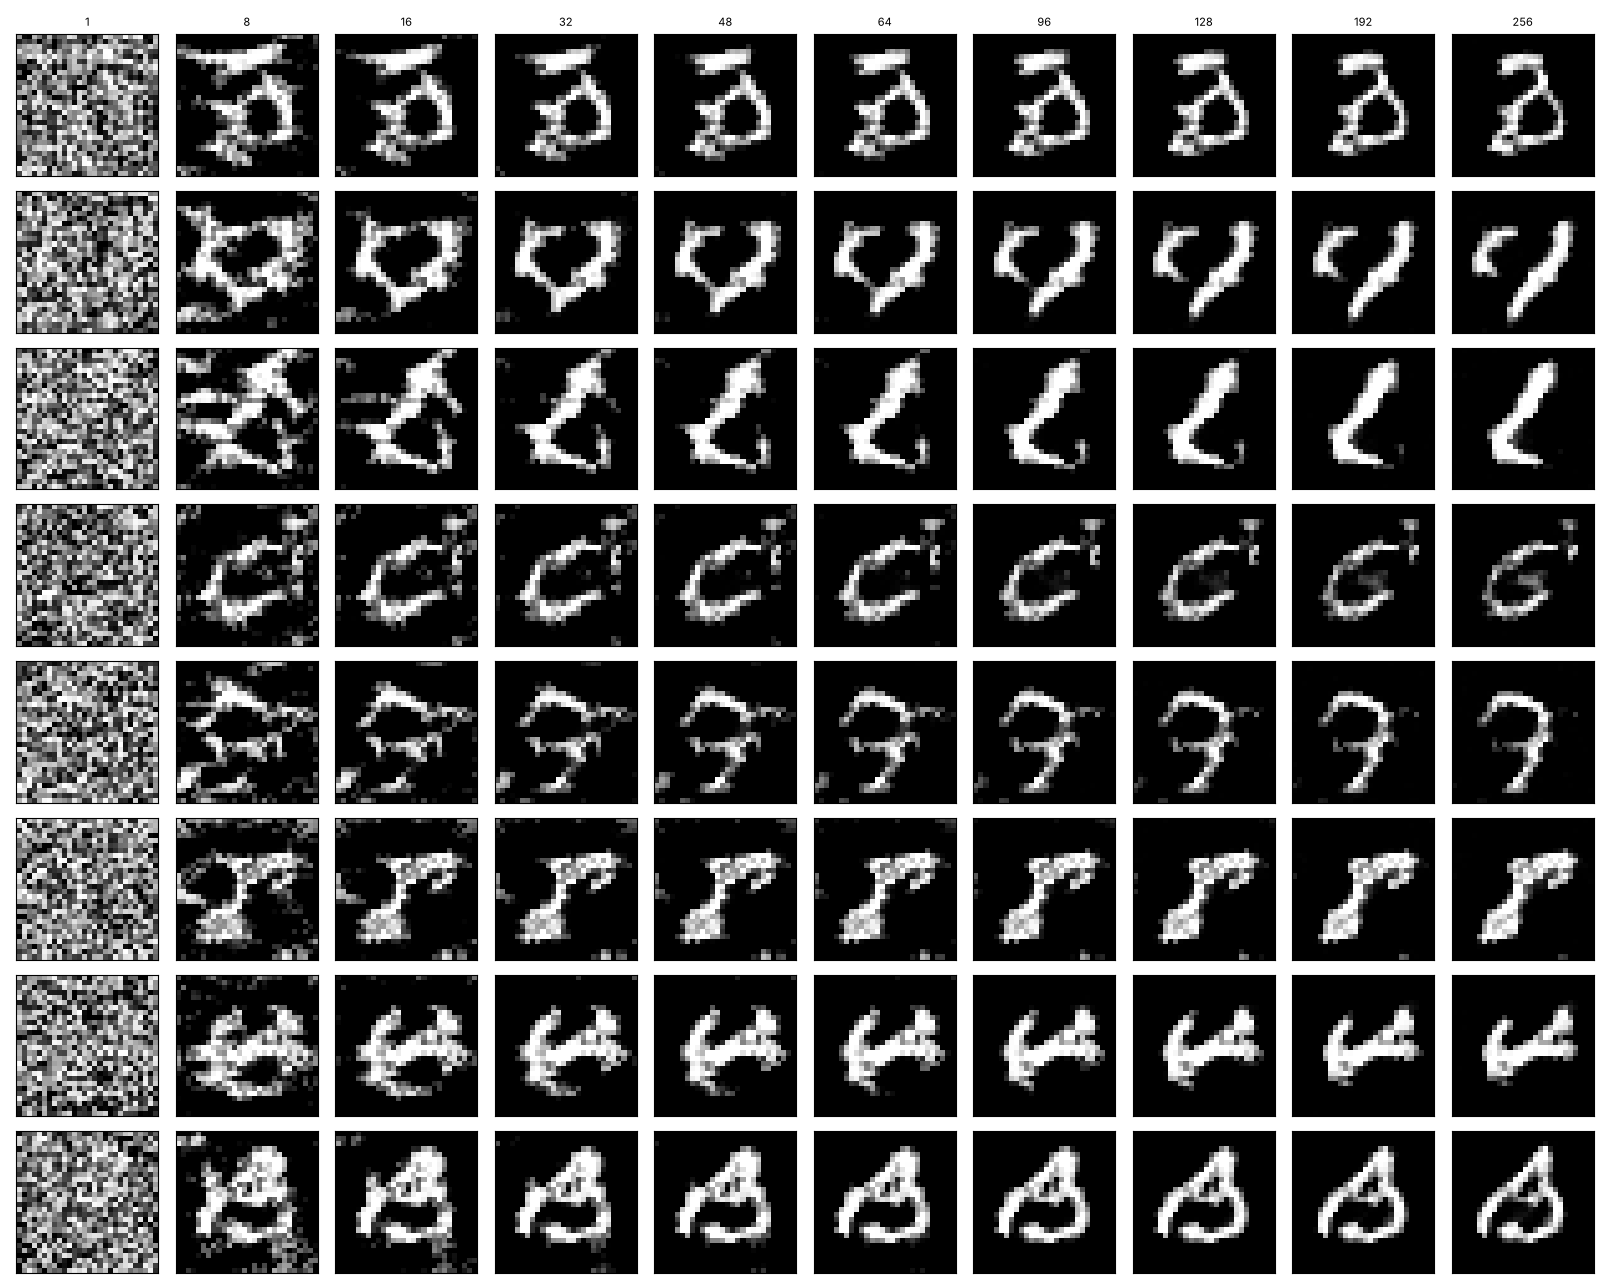
\includegraphics[width=0.95\linewidth]{ebm/mcmc_steps.png}
  \caption{Eight Langevin chains started from uniform noise. Columns are the image after the listed number of steps.}
  \label{fig:ebm-mcmc}
\end{figure}

Step \(1\) is noise. By step \(8\) every chain has a dark background and a bright stroke pattern, and by steps \(32\)--\(48\) most shapes have locked in: the top chain is a \(2\), the third an L-shaped stroke, the fifth a \(7\) with a closed top, and the bottom chain a closed loop. Shapes that have to open or add a stroke take longer. The second chain is a closed V until it opens into a hooked \(7\) around step \(128\), and the fourth is a C until about step \(192\), when it grows an inner stroke and settles toward a \(6\). The sixth and seventh chains are stable by step \(64\) but never become clear digits. Apart from the fourth chain, little changes between steps \(128\) and \(256\) beyond cleaner edges.

So a stable shape takes about \(32\)--\(64\) steps from pure noise, and a recognizable digit, when the chain reaches one, about \(64\)--\(192\). The number depends on the digit: simple strokes and closed loops lock in early, while shapes that need to open or add a stroke keep changing. Only about half of the eight chains end as clear digits, so the model's samples are rougher than its scores on real data suggest. The \(60\) steps used in training are not comparable, because \(95\%\) of those chains start from the replay buffer; from scratch, \(60\) steps only reach the easy shapes.

\subsubsection{Out-of-distribution: random noise}

The score is \(f_\theta\), and lower means less probable. On \(256\) images of each kind:
\begin{center}
\begin{tabular}{lcc}
\toprule
Input & Mean \(f_\theta\) & Spread \\
\midrule
Uniform noise on \([-1,1]\) & \(-15.70\) & all scores in \([-16.11,\,-15.33]\) \\
MNIST test digits & \(0.01\) & std \(0.02\), range \([-0.09,\,0.04]\) \\
MNIST training digits & \(0.00\) & std \(0.03\) \\
\bottomrule
\end{tabular}
\end{center}
A gap of about \(16\) against a real-digit spread of \(0.02\) is exactly what a good anomaly detector should show for unstructured noise.

Real digits sit near zero because of the regularizer in~\eqref{eq:ebm-loss}. The contrastive term only needs \(f(\mathrm{real})\) above \(f(\mathrm{fake})\), and the quadratic penalty is smallest when both are near zero, so the optimizer parks data at about \(0\) and pushes everything else far negative. The score is an unnormalized log-density, so zero just means ``on the scale \(\ell_{\mathrm{reg}}\) chose.''

\subsubsection{Out-of-distribution: image transformations}

The same \(256\) test digits were corrupted three ways: Gaussian noise of scale \(0.3\), clipped to \([-1,1]\); a flip of both spatial axes; and the digit shrunk into the bottom-right corner on a background of \(-1\).
\begin{center}
\begin{tabular}{lc}
\toprule
Transform of the \(256\) test digits & Mean \(f_\theta\) \\
\midrule
Original & \(0.01\) \\
Noise, scale \(0.3\) & \(-0.17\) \\
Flipped vertically and horizontally & \(-0.01\) \\
Shrunk into the corner & \(-0.05\) \\
\bottomrule
\end{tabular}
\end{center}

\begin{figure}[H]
  \centering
  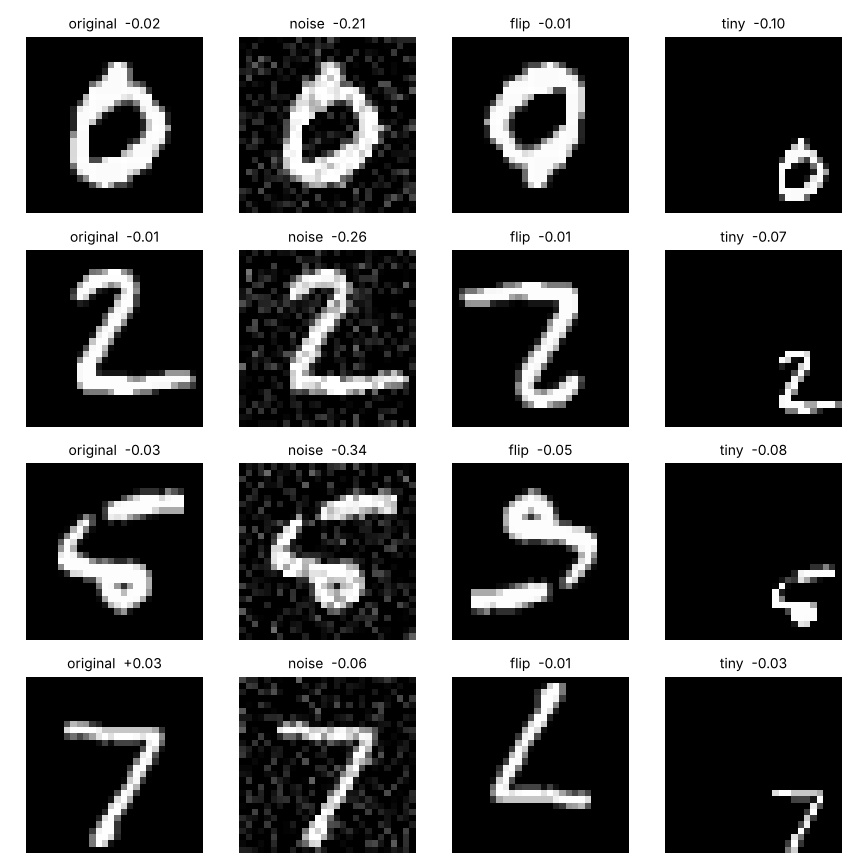
\includegraphics[width=0.62\linewidth]{ebm/transforms.png}
  \caption{Scores \(f_\theta\) for four test digits after the three transformations. Titles are the score of that image.}
  \label{fig:ebm-transforms}
\end{figure}

Noise moves the score by only a few tenths. In Figure~\ref{fig:ebm-transforms} the noisy \(0\) goes from \(-0.02\) to \(-0.21\), the noisy \(5\) from \(-0.03\) to \(-0.34\), and the noisy \(7\) only from \(+0.03\) to \(-0.06\), still inside the range of real scores (the worst test digit in the batch scored \(-0.09\)). Flipped digits are no longer valid instances of their class, yet the batch mean moves by only \(0.02\), and the four flips in the figure by at most \(0.04\). The shrunk digits are the wrong size in the wrong place and move only slightly more: the shrunk \(0\) goes from \(-0.02\) to \(-0.10\), just below the worst real digit, and the shrunk \(7\) from \(+0.03\) to \(-0.03\).

\subsubsection{Is this a good OOD detector?}

It is a good detector of the kind of negatives it was trained against, and a weak detector of anything else.

Unstructured noise sits about \(16\) units below the data with no overlap, so any threshold between \(-1\) and \(-15\) rejects it and keeps ordinary digits. That is what contrastive divergence with short-run Langevin is built for: the negative phase is noise or a short chain that hasn't reached the data yet, so the model learns to score that region low.

Flips and large changes of scale and position are also outside the MNIST generative process, but the scores barely register them. The gap from a real digit to a flipped or shrunk one is a few hundredths, comparable to the spread of real digits (std \(0.02\)), so a threshold that rejected them would also reject ordinary test digits. Pixel noise shifts the mean to \(-0.17\), a real effect, but individual noisy digits still overlap the worst real scores, so the sets are not separable.

The cause is specific. The negative samples never include flipped or rescaled digits, so nothing in~\eqref{eq:cd-grad} raises the energy of an image that still contains plausible local strokes, and the CNN mostly scores those strokes; a flipped \(7\) and a tiny \(2\) both have them. The regularizer then squeezes every in-distribution score toward \(0\), leaving almost no room for a slightly wrong image to stand apart. The model responds to ``stroke on background at roughly the right contrast'' and is insensitive to class identity, orientation, and layout. That is enough to reject pure noise, but not enough for a general out-of-distribution detector.
